\documentclass[11pt,a4paper]{article}

\usepackage[T1]{fontenc}
\usepackage[utf8]{inputenc}
\usepackage[margin=2.5cm]{geometry}
\usepackage{amsmath,amssymb}
\usepackage{graphicx}
\usepackage[dvipsnames]{xcolor}

\usepackage[colorlinks,bookmarksopen,bookmarksnumbered,citecolor=CadetBlue,urlcolor=CadetBlue]{hyperref}
\usepackage{url,apacite}
\usepackage{booktabs}

\usepackage{varwidth}
\setlength{\marginparwidth}{2cm}
\usepackage[colorinlistoftodos]{todonotes}
\makeatletter
\tikzstyle{diaanotestyle} = [
    draw=\@todonotes@currentbordercolor,
    fill=\@todonotes@currentbackgroundcolor,
    line width=0.5pt,
    inner sep = 0.8 ex,
    rounded corners=4pt,align=left,
   ]

\renewcommand{\@todonotes@drawInlineNote}{%
        {\begin{tikzpicture}[remember picture,baseline={(0,0)}]%
            \draw node[diaanotestyle,font=\@todonotes@sizecommand,anchor=base west]{%
               \begin{varwidth}[t]{5cm}
                \raggedright
                \if@todonotes@authorgiven%
                    {\@todonotes@sizecommand \@todonotes@author:\,\@todonotes@text}%
                \else%
                    {\@todonotes@sizecommand \@todonotes@text}%
                \fi
                \end{varwidth}};%
            \end{tikzpicture}}%
       }%
\makeatother  

\title{Empirical critical values for Rasch item fit statistics}

\author{%
    Karl Bang Christensen$^{1}$, Ann-Sophie Buchardt$^{2}$, and Mike Horton$^{3}$\\[2ex]
    \normalsize $^{1}$Section of Biostatistics, Department of Public Health, University of Copenhagen, Denmark\\
    \normalsize $^{2}$Mary Elizabeth’s Hospital, University Hospital Copenhagen, Rigshospitalet, Denmark\\
    \normalsize $^{3}$Psychometric Laboratory for Health Sciences, University of Leeds, UK\\[2ex]
    \normalsize Corresponding author: Karl Bang Christensen, Section of Biostatistics,\\
    \normalsize Department of Public Health, University of Copenhagen,\\
    \normalsize Øster Farimagsgade 5 opg. B, 1353 København K, Denmark. Email: \texttt{kach@sund.ku.dk}
}
\date{}

\begin{document}

\maketitle

\listoftodos

\begin{abstract}
Item fit statistics are very frequently reported as part of Rasch validation studies. Many have an unknown asymptotic distribution, and interpreting what constitutes 'fit' relies on cut-off values that may not always be appropriate. Extensive simulation studies have shown that it is not possible to provide critical fit range values that will apply in all settings. This is a problem for all Rasch validation studies that rely on proprietary software. We introduce an easy-to-use software application that will help in establishing critical values on a case-by-case basis.
\end{abstract}

\noindent\textbf{Keywords:} dichotomous Rasch model, item fit, type I error, asymptotic distribution.

\section{Introduction}

Item fit statistics are arguably the most relevant and certainly the most commonly reported feature in Rasch validation studies. A very wide range of item fit statistics have been developed, but very few are used in practice. The most widely used are (i) the infit and outfit mean square item fit statistics \cite{wright-Stone-1979,Wright-Masters-1982} that are reported in Winsteps \cite{Winsteps} and (ii) the fit residual, Chi-square, and ANOVA item fit statistics in RUMM2030 \cite{Andrich-Sheridan-Luo-2010}. All of these are based on residuals and rely on assumptions about convergence to an asymptotic distribution of the sum of squared Pearson-type standardized residuals. However, this assumption is problematic \cite{Jennings-1986}. 

We study the behavior of the most widely used item fit statistics to see when they produce empirical Type I error rates that are close to the nominal 5\%. This leads us to recommendations regarding reasonable critical values. We do so in a way that reflects the way most users approach evaluation of item fit, i.e.\ looking at the evidence for all items and then evaluating if the item that has the worst fit is a cause for concern when taking the total number of items into account. Thus, we provide guidelines for evaluation of item fit that addresses the issue of multiple testing. 

In the Rasch model, the fit of an item refers to the extent to which an item functions as intended within the context of the overall measurement scale. Sometimes this evaluation entails calculation of a $p$-value, (iii) Standardized residuals where the standardization means that they can be directly compared across items. Furthermore, graphical methods have always been an important part of Rasch analysis: Visual inspection of plots of the observed responses against the expected responses or other fit statistics can also be used to identify items with poor fit.

\emph{Item fit statistics} are a commonly reported feature in Rasch validation studies. Among the wide range of existing item fit statistics, very few are actually used in practice. The most widely used are the fit statistics and the fit of the fit of the fitting and the equipment \cite{wright-Stone-1979,Wright-Masters-1982} reported in the Winsteps software program \cite{Winsteps} and the \emph{fit residual}, \emph{Chi-square} and \emph{ANOVA} item fit statistics reported in the RUMM2030 software program \cite{Andrich-Sheridan-Luo-2010}. 

All of these item fit statistics are based on residuals computed for each person-item interaction. They rely on assumptions about convergence to an asymptotic distribution of the sum of squared Pearson-type standardised residuals. This has been criticised by Karabatsos \cite{Karabatsos-2000}, who provided a critical analysis of the residual fit statistics of the Rasch model and argued:

\begin{quote}
`The faulty statistical properties of the residual fit statistics do not allow either a convenient or a straightforward approach to Rasch fit analysis.'
\end{quote}

More specifically, in mathematical statistics, this assumption from linear models is known to be problematic for non-linear models like the Rasch model, because the residuals have a discrete distribution that depends on the observed value. A consequence of this is that each residual has a unique distribution. In this setting, it is not appropriate to claim that standardised residuals are asymptotically normal or chi-squared \cite{Jennings-1986}. 

Regarding mean squared item residuals, which should ideally be close to 1.0, commonly cited recommendations vary. Bond and Fox \citeyear{Bond-Fox2015} provide rule-of-thumb ranges from 0.8-1.2 to 0.5-1.7, while Linacre \citeyear{Linacre2002} suggests 0.5-1.5 as “productive for measurement” (sic). 

Simple rule-of-thumb critical values for acceptable fit may be inappropriate \cite{Smith-et-al-1998,Wang-Chen-2005}. Critical ranges set using adapted values like $1\pm6/\sqrt{N}$ and $1\pm2/\sqrt{N}$, respectively, are sometimes recommended, as is the use of the Wilson-Hilferty cube-root transformation. However, these do not apply in all settings as illustrated in Monte Carlo simulation studies. Specifically, a common critical range for MNSQs to screen misfitting items fails because of the variability of these across sample sizes. Further, maximum and minimum values were not symmetric around unity, for the outfit with sample sizes around 200, the maximum value could be as large as 2.5. Therefore, commonly used critical ranges were too harsh \cite{Wang-Chen-2005,Seol2016}. Hodge and Morgan \citeyear{Hodge-Morgan-2017} evaluated the stability of infit and outfit "rule-of-thumb" critical values (e.g., 0.7-1.3) in a high-stakes clinical certification exam. Comparing empirical fit statistics with 250 simulated datasets, they found that substantially more values fell within the rule-of-thumb range than within the simulated confidence intervals. This suggests that relying solely on fixed critical values can lead to incorrect conclusions about model-data fit.

Beyond illustrating empirical distributions, Monte Carlo methods have also been used directly in the calculation of item fit statistics. Stone \citeyear{Stone-2000} described a fit statistic based on Monte Carlo that closely approximates a scaled chi-squared random variable and is similar to Yen's \citeyear{Yen-1981} method. Similar methodology was discussed by \citeA{Su-Sheu-Wang-2007} and Wolfe \citeyear{Wolfe-2008} describes an implementation in SAS for estimating critical values for, among other things, the item fit statistics produced by the WINSTEPS computer program.

Wolfe \citeyear{Wolfe-2013} examined the distributions of outfit and infit statistics under a limited number of conditions, and recommended bootstrapping to get adequate critical values. This motivates the method and implementation developed here: Instead of tabulating critical values for a wide range of conditions we outline a general approach for the evaluation of item fit and illustrate an implementation in R for the Rasch \citeyear{Rasch-1960} model for dichotomous items (RMD).

\section{Statistical assumptions and item fit statistics}

Let $X_{vi} \in \{0,1\}$ denote a dichotomous random variable representing a response from person $v = 1,\ldots, N$ to item $i = 1,\ldots,K$. The simplest parametric IRT model is the Rasch \citeyear{Rasch-1960} model for dichotomous items (RMD) also known as the 1PL model, 
\begin{equation}
\label{RMD}
P(X_{vi}=x|\theta_v=\theta)
=\frac{\exp(x(\theta-\delta_i))}{1 + \exp(x(\theta-\delta_i))}.
\end{equation}

In the Rasch model the parameters $\delta_1,\ldots,\delta_k$ that can be interpreted as item difficulties and estimates $\hat\delta_1,\ldots,\hat\delta_k$ can be computed in several ways \cite{Christensen-2013,Robitzsch-2021}, but typically the choice of estimation procedure is dictated by the choice of software. For users of proprietary software this means this means: marginal maximum likehood (MML) estimation for ConQuest \cite{Adams-Wu-Cloney-Wilson-2020} users; pairwise conditional estimation (PCML; \citeNP{Zwinderman-1995,Andrich-Luo-2003}) for RUMM \cite{Andrich-Sheridan-Luo-2010} users; joint maximum likelihood (JML) estimation for Winsteps \cite{Winsteps} users. 

Estimates $\hat\theta_1,\ldots,\hat\theta_N$ of the person parameters $\theta_1,\ldots,\theta_N$ can be computed using maximum likelihood (ML), weighted maximum likelihood (WML; \citeNP{Warm-1989}) and other methods \cite{Kreiner-Christensen-2013}. Again, the choice of estimator is often dictated by the choice of software.

After observing data $(x_{vi})$ and estimating item and person parameters, the issue of model fit boils down to whether or not the observed data is consistent with the data generating mechanism

\begin{equation}
\label{IRThat}
P(X_{vi}=x_{vi}|\theta_v=\hat\theta_v),
\end{equation}
for all $v = 1,\ldots,N$.

This question is typically addressed using statistical tests and tests with a specified alternative, e.g., 'misfit is due to item $i_0$', are usually used.


\section{Item fit statistics}

This section describes three item fit statistics that are widely used in Rasch analysis. Let for $v=1,\ldots,N$ and $i=1,\ldots,K$
$$
E_{vi} = E(X_{vi} | \theta_v = \hat\theta_v)
$$ 
and 
$$
V_{vi} = V(X_{vi} | \theta_v = \hat\theta_v)
$$
denote the expected value and variance, respectively, of the item responses conditional on the estimated value $\hat\theta_v$ of $\theta_v$.

Let $z_{vi}$ denote the standardized residuals, that is,
$$
z_{vi} = \frac{x_{vi} - E_{vi}}{\sqrt{V_{vi}}}
$$

\subsection{Outfit}

The outfit item fit statics for the $i=1,\ldots,K$ items is defined as
\begin{equation}
u_i = \frac1N\sum_{v=1}^N z_{vi}^2.
\label{outfit}
\end{equation}

\subsection{Infit}

The infit item fit statistics for the $i=1,\ldots,k$ items is defined as
\begin{equation}
v_i = \frac{z_{vi}^2}{\sum_{v = 1}^N V_{vi}}.
\label{infit}    
\end{equation}


The item fit statistics (\ref{infit}) and (\ref{outfit}) have no established null distribution though false claims that they do can be found in early Rasch literature \cite{Wright-Panchapakesan-1969,wright-Stone-1979}. Transformations have been proposed and implemented.

\subsection{Transformations}

Let for $i=1,\ldots,K$
$$
q_i^2 = \frac{1}{N^2} \sum_{v=1}^N \frac{C_{vi}}{V_{ni}^2} - \frac1N,
$$
where
$$
C_{vi} = E_{vi}^4 (1 - E_{vi}) + (1-E_{vi})^4 E_{vi}.
$$
It has been suggested that the Wilson-Hilferty \citeyear{Wilson-Hilferty-1931} cube-root transformations
\begin{equation}\label{wilson-hilferty-OUT}
t_{u,i} = \frac{3u_i^{\frac{1}{3}} - 1}{q_i} + \frac{q_i}{3}
\end{equation}
and
\begin{equation}\label{wilson-hilferty-IN}
t_{v,i} = \frac{3v_i^{\frac{1}{3}} - 1}{q_i} + \frac{q_i}{3}
\end{equation}
yield distributions that approximate a $t$ distribution \cite[Table 5.4a, p.100]{Wright-Masters-1982}. However, this claim rests on the false assumption that the item fit statistics (\ref{infit}) and (\ref{outfit}) follow a $\chi^2$ distribution. Another transformation of the outfit test statistic is reported in the software package RUMM \cite{Andrich-Sheridan-Luo-2010}. This transformation is based on using the ratio $S_i/f$ where
\begin{equation}
S_i = \sum_{v = 1}^N z_{vi}^2.
\label{S}
\end{equation}
This ratio is argued to be approximately chi-square distributed on $f$ degrees of freedom using an ad hoc derivation that, in the notation of this paper, amounts to $N\cdot k$ data points minus $N+k-1$ estimated parameters with each item contributing equally yielding $f=(Nk-N-k+1)/k$. Using the approximation
\begin{equation}
V(\log(S_i/f))\simeq\frac1{f^2}{V(S_i)}
\end{equation}
the test statistic FitResid defined as 
\begin{equation}
s_i=\frac{\log(S_i/f)}{\sqrt{V(\log(S_i/f))}}
=\frac{f(\log(S_i)-\log(f))}{\sqrt{V(S_i)}}
\label{FitResid}
\end{equation}
is argued to have a symmetrical distribution with mean zero and variance one. The item fit residual is considered to be sensitive towards a deviation from the requirement of equal discrimination, and $\pm2.5$ are commonly accepted thresholds. 

\subsection{Other item fit statistics}

The McKinley and Mills \citeyear{McKinley-Mills-1985} likelihood ratio $G^2$ and Yen's \citeyear{Yen-1981} Q1 have both been argued to have an approximate $\chi^2$ distribution. Computing one of these fit statistics for each of the $K$ items and reporting the largest observed value will inherently lead to type I errors. 

The Molenaar \citeyear{Molenaar-1983} item fit statistic $U$ for evaluating item fit in the RMD summarizes trends in residuals calculated in different score groups derived by partitioning the score range into three intervals. Molenaar argued that $U$ has an asymptotic standardized normal distribution under the Rasch model and that large positive or negative values for an item indicates that the discrimination is stronger or weaker, respectively, than what is assumed by the Rasch model. 

\subsection{Summary}

Published Rasch validation studies will very often report an item fit statistic for each of the items in a scale and then report on the item (or items). Trust in the null distribution and a reasonable strategy for addressing multiple testing is needed. 

\section{Methods}

Inspired by earlier work \cite{Stone-2000,Su-Sheu-Wang-2007,Wolfe-2008,Hodge-Morgan-2017} we propose the following general approach:

\begin{enumerate}
\item Given estimates $\delta_1,\ldots,\delta_K$ and $\theta_1,\ldots,\theta_N$ simulate $B$ data sets using the data generating mechanism (\ref{IRThat}) and, for each of these:
\begin{enumerate}
\item Estimate $\delta_1^{(s)},\ldots,\delta_K^{(s)}$ and $\theta_1^{(s)},\ldots,\theta_N^{(s)}$ using an estimation method of choice;
\item compute the item fit statistic of choice $Z_i^{(s)}$ for each item;
\item compute $L^{(s)}=\min\{Z_i^{(s)}:i=1,\ldots,K\}$; and
\item compute $U^{(s)}=\max\{Z_i^{(s)}:i=1,\ldots,K\}$.
\end{enumerate}
\item Evaluate percentiles for $(L^{(s)})_{s=1,\ldots,B}$, $(U^{(s)})_{s=1,\ldots,B}$, or both, as appropriate.
\end{enumerate}

This approach applies to any estimation method and, for this reason, can be used to study the empirical distribution of item fit statistics from proprietary software. In this paper we present a software implementation that generates these empirical distributions. It is part of the \texttt{RASCHplot} package which is available as a free package for the R software environment \cite{R}. In addition, we have supplemented the R code with a shiny app \cite{shiny} to provide a web interface. Shiny is an open source R package that provides an elegant and powerful web framework for building web applications using R \cite{beeley2013}. The ‘app’ can be interacted with by entering data, running functions with user-specified settings to plot figures, and downloading the resultant figures in a variety of formats.

%\todo[inline]{Følgende er en forkortet og mindre R-teknisk version af den i R-afsnittet}
The computational algorithm relies on repeated random sampling to obtain a sampling distribution for an item fit statistic of interest, in particular, the outfit, infit, or item fit residual. From the imported item and person parameter estimates $\hat\delta_1,\ldots,\hat\delta_k$ and $\hat\theta_1,\ldots,\hat\theta_k$ conditional probabilities for item responses are computed under the model \eqref{RMD}. The probabilities are stored in a matrix as follows:
\begin{equation}
\boldsymbol{\hat{P}}
=
\left[\hat{P}_{vi}\right]_{\substack{v=1,\ldots,N \\ i=1,\ldots,K}}
=
\left[P(x_{vi}=1 \mid \theta_v=\hat\theta_v; \delta_i=\hat\delta_i)\right]_{\substack{v=1,\ldots,N \\ i=1,\ldots,K}}.
\label{probability-matrix}
\end{equation}
Then, for each cell in the matrix of probabilities, a random number is generated from a uniform distribution $p^{(l)}_{vi} \sim \mathcal{U}[0,1]$ and we define $x^{(l)}_{vi}=1$ if $\hat{P}_{vi} > p^{(l)}_{vi}$ and $x^{(l)}_{vi}=0$ otherwise. This way we generate a data matrix  $\mathbf{x}^{(l)}$, $l=1,2,\ldots$, of item responses.
For each sample, we estimate the parameters of a parametric IRT model using an estimation method of the users choice. Furthermore, the item fit statistics presented above are computed. Finally, from a suitable number of repetitions, we obtain an estimate of the sampling distribution for the minimum and maximum item fit statistics, $(L^{(s)})_{s=1,\ldots,B}$ and $(U^{(s)})_{s=1,\ldots,B}$, respectively. Four estimation  methods are available for the item parameter estimation through the \texttt{RASCHplot} package, namely,
PCML \cite{sirt}, CML \cite{erm}, JML  \cite{tam}, and MML \cite{tam}.
Two estimation methods are available for the person parameter estimation, namely WML and ML \cite{sirt}. 

A key feature of the proposed method is that we can visualize the estimated sampling distribution of an item fit statistic. We can produce a density plot of the sampling distribution of an item fit statistic, that is, for a sampled minimum $(L^{(s)})_{s=1,\ldots,B}$ or maximum $(U^{(s)})_{s=1,\ldots,B}$ item fit statistic of choice. This is possible for any the item fit statistics presented above. Percentiles representing critical values can be indicated in the figures. For example, the values 2.5\% and 5\% could be reasonable for the minimum while 95\% and 97.5\% could be reasonable for the maximum. The \texttt{RMDitemfit} Shiny app generates a sampling distribution for different Rasch item fit statistics and visualizes empirical critical values. The app is available free of charge (\url{https://shiny.sund.ku.dk/RMDitemfit/}) and can also be found through the \texttt{RASCHplot} package so that users can run the app locally using \texttt{RASCHplot::app("RMDitemfit")}.


\section{Example with dichotomous data: AMTS data}

This example uses the responses of 197 persons to the ten questions of the Abbreviated Mental Test Score \cite[AMTS]{hodkinson72}. One point is given for each correct answer; a score of 6 or less suggests that the patient has some mental impairment. Table \ref{tab:amtsfit} shows item locations and three item-fit evaluations

\begin{table}[h!]
    \centering
    \caption{Item locations and three item-fit evaluations for the abbreviated mental test score.} \label{tab:amtsfit}
    \begin{tabular}{lrrrrr}
    \\
    \toprule
             &          &    & RUMM     & \multicolumn{2}{c}{Winsteps}\\
    Item     & $\delta$ & SE & FitResid & Outfit & Infit\\
    \midrule
    Age      & -0.68 & 0.22 & -1.27 & 0.63 & 0.84 \\
    Time     &  0.08 & 0.20 &  0.57 & 1.00 & 0.98 \\
    Address  &  1.91 & 0.20 &  0.62 & 1.05 & 1.12 \\
    Name     & -0.62 & 0.22 & -0.65 & 0.75 & 0.87 \\
    Year     &  0.16 & 0.20 & -1.30 & 0.70 & 0.85 \\
    Dob      & -1.69 & 0.27 & -0.46 & 0.72 & 0.99 \\
    Month    &  0.46 & 0.20 & -2.65 & 0.57 & 0.66 \\
    Firstww  & -0.12 & 0.21 &  1.35 & 1.18 & 1.14 \\
    Monarch  &  0.17 & 0.20 & -0.28 & 0.85 & 0.93 \\
    Countbac &  0.34 & 0.20 &  2.30 & 1.34 & 1.25 \\
    \bottomrule
    \end{tabular}
\end{table}

For all three fit statistics, the value is seen to be smallest for the item 'Month' and largest for the item 'Countbac'. Thus, the three values are in agreement (and with respect to the item 'Month', they also agree with an earlier reported analysis using comparison of observed and expected item-restscore correlations \cite{Christensen-Kreiner-2013} and graphical evaluation of item fit \cite{Buchardt2023VisualizingR}). 

\subsection{FitResid}

Conventional rules-of-thumb would flag the item 'Month' as an anomaly. The question is whether the observed values actually constitute an anomaly. To answer this question, we rely on the approach outlined in the methods section. Minimum values below -2.65 occurred in 16\% of the simulated data sets and thus the observed value does not constitute evidence against the Rasch model. On the other hand maximum values above 2.30 occurred only in 1\% of the simulated data sets and for thus this observed value could be interpreted as evidence against the Rasch model. Figure \autoref{fig:amtsFitResidMinMax} shows the empirical distribution of the smallest (left panel) and largest (right panel) values of the ten FitResid values computed in each of $B=2000$ simulated data sets. 

\begin{figure}[h!]
    \centering
    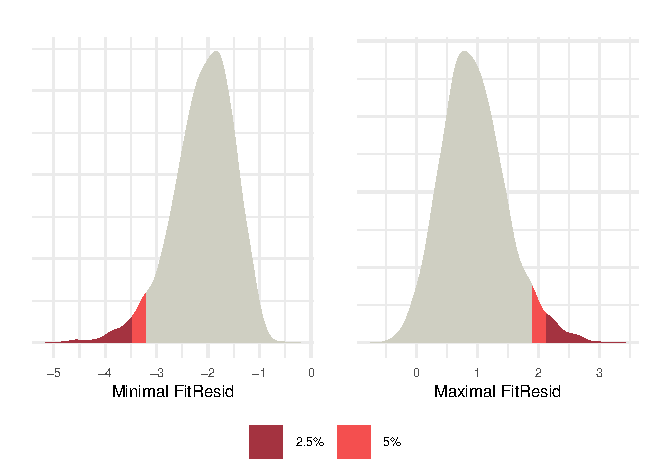
\includegraphics{amtsFitResid.pdf}
    \caption{Empirical critical values for minimum (left) and maximum (right) item fit residual values for the AMTS.}
    \label{fig:amtsFitResidMinMax}
\end{figure}

Minimum values below -3.47 occur in 2.5\% of the simulated data sets and that minimum values below -3.19 occur in 5\% of the simulated data sets. Similarly, maximum values above 2.13 occur in 2.5\% of the simulated data sets and maximum values above 1.89 occur in 5\% of the simulated data sets.

\subsection{Outfit}

Minimum values below 0.57 occurred in 57\% of the simulated data sets and thus the observed value does not constitute evidence against the Rasch model. Maximum values above 1.34 occurred only in 4\% of the simulated data sets, so this observed value could be interpreted as mild evidence against the Rasch model. Figure \autoref{fig:amtsOutfitMinMax} shows the empirical distribution of the smallest (left panel) and largest (right panel) values computed in each of $B=2000$ simulated data sets. 

\begin{figure}
    \centering
    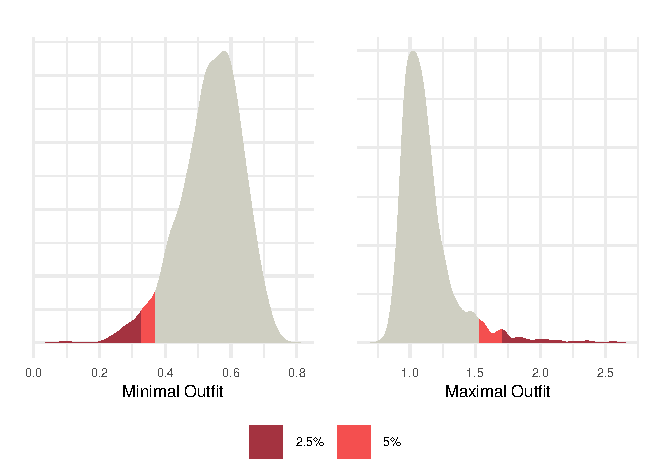
\includegraphics{amtsOutfit.pdf}
    \caption{Empirical critical values for minimum (left) and maximum (right) outfit item fit statistics for the AMTS.}
    \label{fig:amtsOutfitMinMax}
\end{figure}

Again, the values that occur less than 5\% of the times and values that occur less than 2.5\% of the times are indicated.

\subsection{Infit}

Minimum values below 0.66 occurred in only 1\% of the simulated data sets and thus the observed constitutes evidence against the Rasch model. Maximum values above 1.34 occurred only in 3\% of the simulated data sets, so this observed value could be interpreted as mild evidence against the Rasch model. Figure \autoref{fig:amtsInfitMinMax} shows the empirical distribution of the smallest (left panel) and largest (right panel) values computed in each of $B=2000$ simulated data sets. 

\begin{figure}
    \centering
    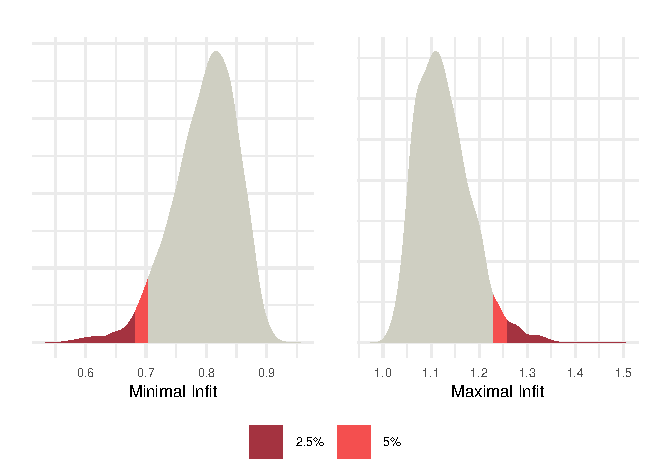
\includegraphics{amtsInfit.pdf}
    \caption{Empirical critical values for minimum (left) and maximum (right) infit item fit statistics for the AMTS.}
    \label{fig:amtsInfitMinMax}
\end{figure}

Again, the values that occur less than 5\% of the times and values that occur less than 2.5\% of the times are indicated.

\section{Discussion}

Here we describe an online interface, implemented in R, that allows users to estimate empirical critical values for item fit statistics under the conditions of their own data, rather than relying on a single fixed cut-off. Confidence intervals generated via simulation provide a more nuanced and accurate assessment of item fit than rule-of-thumb ranges, since they naturally accommodate sample size and the alignment between item difficulty and person ability. We offer this as a resource to help put observed fit statistics into context, in order to determine whether an apparent anomaly is statistically relevant.

Specifically, we propose a method for empirically studying the behavior of item fit statistics to see when they produce empirical Type~I error rates that are close to the nominal 5\%. Doing so yields critical values that vary depending on conditions like sample size, test length, response format, and targeting, and we provide an implementation in R based on parametric bootstrap for this purpose. We further discuss how this implementation is useful for the evaluation of item fit and address the issue of multiple testing in the context of the wide variation in the number of items across instruments.

This matters because the use of a single critical value for misfit diagnosis, applied uniformly across different conditions, leads to both the overdetection and underdetection of misfit. Karabatsos \cite{Karabatsos-2000} provided a critical analysis illustrating that the task of Rasch fit analysis is not as simple and straightforward as it appears to be: the faulty statistical properties of the residual fit statistics do not allow either a convenient or a straightforward approach to Rasch fit analysis. For any of these fit statistics, using a single minimum critical value for misfit diagnosis across testing situations that vary in sample and test properties leads to both the overdetection and underdetection of misfit.

Bootstrap-based approaches to this problem are not new: Wolfe \citeyear{Wolfe-2013} describes three implementations of the bootstrap procedure for evaluating person and item fit. A parallel line of work exists for person fit: Dimitrov and Smith \todo[inline]{confirm authors/reference} and, in the context of person fit, Magis et al.\ \todo[inline]{confirm reference} adapted a general approach proposed by Snijders (2001) \todo[inline]{confirm reference} to correct infit and outfit indices, comparing the corrected indices to their classical versions in a simulation study; the correction was found to control Type~I errors while substantially increasing power to detect specific misfitting response patterns.

Karabatsos also advocated the use of residual-free Rasch fit statistics based on the number of Guttman response errors, and for the dichotomous Rasch model Kreiner and Christensen studied exact tests based on the same principle \todo[inline]{confirm this description and add citation}. Empirically, the standard deviations of the infit and outfit mean squares become smaller as the sample size increases. Simulation studies have shown that the means of $t$-transformed infit and outfit item fit statistics are very close to zero but have standard deviations considerably smaller than one, and that these standard deviations become smaller still as the number of items increases \todo[inline]{cite source(s) for these two empirical findings}.

Item fit statistics with known asymptotic properties \cite{Christensen-Kreiner-2013,Muller-2020,Johansson2025} exist and have been implemented in R \cite{iarm}, but the use of residual fit statistics with faulty statistical properties persists. Until such time as item fit statistics with known asymptotic properties are commonly used, it would be helpful for practitioners to have guidelines for interpreting the residual fit statistics produced by the current major Rasch software packages. In a related vein, Rost and von Davier \citeyear{Rost-vonDavier-1994} proposed a probabilistic measure of item fit for dichotomous and ordinal Rasch models based on the likelihood of the item response patterns, providing both a descriptive measure of the degree of disturbance in the data and a measure for statistical inference about the fit of single items.

\todo[inline]{write part about how this paper and application are also relevant to apply to pre-existing research where fit statistics for a scale/PROM have been presented}

\bibliographystyle{apacite}
\bibliography{biblio.bib}

\end{document}
